\documentclass[11pt]{article}

\usepackage[margin=1in]{geometry}
\usepackage{amsmath,amssymb}
\usepackage{booktabs}
\usepackage{threeparttable}
\usepackage{graphicx}
\usepackage{caption}
\usepackage{setspace}
\usepackage[round,authoryear]{natbib}
\usepackage[hidelinks]{hyperref}
\usepackage{xcolor}

\captionsetup{font=small,labelfont=bf}
\makeatletter
\newcommand\inputtable[1]{\@@input #1 }
\makeatother

\setstretch{1.25}

\newcommand{\dirBeta}{-0.067}\newcommand{\dirHit}{52.8}\newcommand{\dirBase}{54.9}\newcommand{\dirBetaTest}{-0.008}\newcommand{\dirPTest}{0.723}
\newcommand{\nPlaceboOld}{115}\newcommand{\nPlaceboNew}{86}

\title{Downside Volatility Predicts Risk, Not Returns:\\ Out-of-Sample Evidence from Korea and the U.S.}
\author{Park Dong Gyu\thanks{Independent researcher. E-mail: \href{mailto:parkdong1015@gmail.com}{parkdong1015@gmail.com}. This paper was prepared with substantial assistance from a generative AI tool; see the declaration at the end of the paper.}}
\date{This version: September 2026}

\begin{document}
\maketitle

\begin{abstract}
\noindent
We revisit the asymmetric relation between downside price moves and future volatility, and the many attempts to turn the same asymmetry into return forecasts, in Korea and the United States under a common design with internally frozen trading rules, a held-out 2021--2026 test period, and multiple-testing corrections. Downside realized semivariance predicts future upside, downside, and total variance, while upside semivariance does not; the effect survives Holm adjustment in both markets over 2005--2020 and replicates out of sample in the U.S.\ but not in Korea. Contrary to the common presumption, the leverage effect does not strengthen in turbulent regimes; in the U.S.\ it weakens. By contrast, directional asymmetry measures built from daily returns---monthly relative signed jump variation and weekly realized skewness---carry no return information beyond short-term reversal: their rank correlation with the same-period return is 0.76--0.87, and their Fama--MacBeth coefficients vanish once reversal is controlled for. The dominant direction of tomorrow's variation cannot be forecast better than a naive baseline, and stock-level forecasts of upside and downside semivariance rank stocks almost identically. A cross-country difference-in-differences analysis of the 2023--2025 Korean short-sale ban finds no change in the cross-sectional pricing of these measures, although the test has limited power. Overall, asymmetry is useful for forecasting risk, not returns.

\bigskip
\noindent\textbf{Keywords:} realized semivariance; leverage effect; realized skewness; short-term reversal; short-sale ban; out-of-sample testing; multiple testing; Korea stock market

\noindent\textbf{JEL:} C22, C58, G12, G14, G17
\end{abstract}

\newpage

% ===========================================================================
\section{Introduction}
% ===========================================================================

Negative returns are followed by higher volatility than positive returns of the same size. This asymmetry, usually called the leverage effect \citep{black1976,christie1982}, is one of the most robust facts in empirical finance, and modern realized-measure models exploit it directly: heterogeneous autoregressive (HAR) models augmented with past negative returns \citep{corsi2009,corsireno2012} and models that split realized variance into upside and downside semivariance \citep{bns2010,pattonsheppard2015} forecast volatility better than symmetric benchmarks.

A parallel literature asks whether the same directional information predicts \emph{returns}. Realized skewness and signed jump measures computed from high-frequency data have been reported to forecast the cross-section of returns \citep{amaya2015}, and related lottery-type characteristics such as maximum daily return and idiosyncratic volatility have been linked to low subsequent returns \citep{ang2006,bali2011}. When high-frequency data are unavailable, such measures can only be approximated with daily returns, and how much of their information survives the approximation is an empirical question. At the same time, the replication literature has shown that many published return predictors weaken or disappear once multiple testing and out-of-sample evaluation are taken seriously \citep{hlz2016,hxz2020}.

This paper puts both questions---does downside volatility predict risk, and does it predict returns---under a single design in two markets, Korea and the United States. Every trading rule is fixed on a development sample and frozen before a held-out test period (2021--2026) is opened, and every family of hypotheses is reported with Holm and Benjamini--Hochberg adjustments. The paper is a replication and validation study; it does not propose a new anomaly. Its contributions are the following.

\paragraph{1. The volatility asymmetry replicates, with a twist.} Downside semivariance predicts future upside, downside, and total variance, whereas upside semivariance has no total effect. The result survives multiple-testing adjustment in both markets over 2005--2020 and replicates in the U.S.\ test sample; it does not survive adjustment in the shorter and unusually volatile Korean test sample. Log-LHAR forecasts reduce out-of-sample QLIKE loss by 3.6\% (U.S.) and 3.8\% (Korea) relative to HAR. Contrary to the common presumption that the leverage effect is stronger in turbulent markets, its interaction with a turbulent-regime indicator is negative in the U.S.\ ($t=-4.62$) and insignificant in Korea, consistent with saturation when volatility is already high.

\paragraph{2. Daily directional asymmetry measures are reversal in disguise.} Monthly relative signed jump variation (RSJ) and weekly realized skewness computed from daily returns have rank correlations of 0.76--0.87 with the same-period return. Their apparent predictive power disappears once short-term reversal is controlled for. We stress that this is a statement about the daily approximation, not a failed replication of the high-frequency results in \citet{amaya2015}.

\paragraph{3. Magnitude is predictable; direction is not.} Whether tomorrow's variation will be dominated by up or down moves cannot be forecast better than always predicting the sample majority. At the stock level, forecasts of next-month upside and downside semivariance are informative about magnitude but rank stocks almost identically (rank correlation 0.98--0.997), so a strategy that buys stocks with high predicted upside volatility does not outperform.

\paragraph{4. The 2023--2025 Korean short-sale ban.} In a cross-country difference-in-differences design with the U.S.\ as the control market, the ban did not change the cross-sectional return slopes of RSJ, realized skewness, maximum return, or idiosyncratic volatility, including against a placebo distribution purged of earlier Korean bans. Because these slopes were close to zero before the ban, the test has limited power; we report it as a carefully documented null result.

We also document why several strategies that looked strong in the development sample failed in the test sample. In 2021--2026, days classified as turbulent delivered the \emph{highest} returns (sharp V-shaped rebounds and the 2025--2026 Korean rally), so rules that exit the market in turbulent regimes forfeited much of the test-period return, whereas volatility targeting, which only scales exposure down, did not.

Section~\ref{sec:data} describes the data and the research protocol. Sections~\ref{sec:vol}--\ref{sec:ban} present the four sets of results. Section~\ref{sec:practice} discusses implications for practice and Section~\ref{sec:conclusion} concludes. The appendices report the audit trail of frozen rules, the full multiple-testing results, and exploratory intraday evidence.

% ===========================================================================
\section{Related literature}
% ===========================================================================

\paragraph{Asymmetric volatility.} The negative correlation between returns and subsequent volatility has been attributed to financial leverage \citep{black1976,christie1982} and to volatility feedback. \citet{corsi2009} introduced the HAR model, and \citet{corsireno2012} added lagged negative returns at daily, weekly, and monthly horizons (LHAR).

\paragraph{Realized semivariance.} \citet{bns2010} decompose realized variance into upside and downside semivariance. \citet{pattonsheppard2015} show that downside semivariance is far more informative about future volatility than upside semivariance. Our daily-frequency test follows their specification.

\paragraph{Realized skewness and lottery-type stocks.} \citet{amaya2015} report that weekly realized skewness computed from intraday data negatively predicts next-week returns, and \citet{sim2016} reports a similar relation for Korean stocks using intraday data. \citet{bali2011} and \citet{ang2006} document low returns on stocks with high maximum daily returns and high idiosyncratic volatility.

\paragraph{Short-term reversal.} Weekly and monthly returns reverse in the cross-section \citep{jegadeesh1990,lehmann1990}; \citet{nagel2012} links reversal profits to liquidity provision.

\paragraph{Short-sale restrictions.} Binding short-sale constraints may delay the incorporation of negative information \citep{miller1977,diamondverrecchia1987}. The 2008 bans have been studied extensively \citep{beberpagano2013,boehmer2013}. Korea has banned short selling four times: from October 2008 (lifted for non-financial stocks in June 2009 but for financial stocks only in November 2013), from August to November 2011, from March 2020 (lifted in May 2021 only for constituents of the KOSPI 200 and KOSDAQ 150 indices), and for all stocks from November 2023 to March 2025. For the 2008 ban, \citet{eom2021} find no evidence that the ban raised volatility or reduced liquidity; for the 2021 partial reopening, \citet{kimkim2024} find that permitting short sales improved price efficiency without significant effects on volatility. We study the most recent ban, and ask a different question: whether it changed the cross-sectional return predictability of downside-risk signals.

\paragraph{Volatility management and replication.} \citet{moreiramuir2017} report that volatility-managed portfolios earn higher Sharpe ratios; \citet{cederburg2020} find that this advantage is fragile out of sample. \citet{hlz2016} and \citet{hxz2020} discuss multiple testing and replication in asset pricing.

% ===========================================================================
\section{Data and research protocol}\label{sec:data}
% ===========================================================================

\subsection{Data}

\paragraph{Indices and ETFs.} Volatility forecasts use daily open, high, low, and close prices of the S\&P 500 index (\texttt{\^{}GSPC}) and the KOSPI index (\texttt{\^{}KS11}) from 2000 to September 2026. Daily variance is the \citet{parkinson1980} range estimator (in \%$^2$); semivariances use squared daily log returns split by sign. Allocation backtests trade the SPY ETF and the KODEX 200 ETF (069500.KS; available from 2007) using dividend-adjusted prices.

\paragraph{U.S.\ stocks.} The U.S.\ cross-section is drawn from historical S\&P 500 constituents (1,008 distinct firms), with daily prices from Yahoo Finance. Firms that were later delisted or acquired are often unavailable: over 2000--2026, 22.1\% of a month's constituents are missing on average (at most 40.6\%); within the 2010--2020 development sample the share is 19.7\% (at most 26.7\%), and in the test sample 5.5\%. \emph{The U.S.\ cross-sectional results should therefore be read as results for a sample of surviving large-capitalization stocks}, not for the full S\&P 500 or the U.S.\ market. Size is proxied by dollar trading volume because historical market capitalization is unavailable.

\paragraph{Korean stocks.} The Korean cross-section uses the Korea Exchange (KRX) Open API, which returns all listed KOSPI stocks on each trading day from 2010, so delisted firms are included. Each month we keep the 200 largest common stocks by market capitalization as a proxy for the KOSPI 200 (1,251 distinct firms over the sample). Returns are price returns computed from the exchange's adjusted daily change and \emph{exclude dividends}. The resulting panel has 39,950 stock-months (U.S.: 112,809).

\paragraph{Intraday data.} For exploratory analyses we use 60-minute bars for about three years (2023--2026) and 5- and 10-minute bars for 60 trading days, for the two indices, the two ETFs, and 50 large stocks per market. The 50 stocks are a fixed list of \emph{currently} large firms, so the intraday stock panels are subject to look-ahead selection. Korean intraday bars end before the closing auction.

\paragraph{Costs.} We assume one-way costs of 2 bps (SPY), 8 bps (KODEX 200), 5 bps (U.S.\ stocks), and 10 bps (Korean stocks), plus a Korean sell-side transaction tax. The tax is fixed at 0.18\% (its 2024 level), whereas the statutory rate for KOSPI stocks, including the special rural development tax, was 0.30\% before June 2019, 0.25\% in 2019--2020, 0.23\% in 2021--2022, 0.20\% in 2023, 0.18\% in 2024, 0.15\% in 2025, and 0.20\% again from 2026. Costs of Korean stock strategies are therefore understated in the development sample, which biases \emph{in favor of} finding net profits; none of our conclusions relies on net profits being positive.

Table~\ref{tab:sample} summarizes the samples. Index returns were higher in the test period than in the development period in both markets, and Korean index volatility rose from 20\% to 28\% per year.

\begin{table}[!htbp]
\centering
\begin{threeparttable}
\caption{Sample summary}\label{tab:sample}
\small
\begin{tabular}{lcccc}
\toprule
 & \multicolumn{2}{c}{U.S.} & \multicolumn{2}{c}{Korea} \\
\cmidrule(lr){2-3}\cmidrule(lr){4-5}
 & Development & Test & Development & Test \\
\midrule
\inputtable{tables/t_sample.tex}
\bottomrule
\end{tabular}
\begin{tablenotes}\footnotesize
\item Panel A: S\&P 500 and KOSPI daily log returns; development 2005--2020, test 2021--September 2026. Panel B: stock-months with a valid signal and next-month return; development 2010--2020. ``Constituents missing'' is the share of S\&P 500 members in a month without price data (none for Korea, where the exchange data include delisted firms). Panel C reports means and standard deviations pooled over development-sample stock-months; the column headers of Panels A and B do not apply to it.
\end{tablenotes}
\end{threeparttable}
\end{table}

\subsection{Sample splits}

Index-level analyses (volatility forecasting, allocation) use 2005--2020 as the development sample, with 2000--2004 as burn-in for regime estimation. Cross-sectional analyses use 2010--2020, a start date chosen before any cross-sectional result was computed because the KRX API begins in 2010 and U.S.\ survivorship is most severe earlier. The test sample is January 2021 to September 2026 for all analyses. All intraday data fall in the test period and are treated as exploratory.

The Korean test sample contains the 2023--2025 short-sale ban: 17 of its 69 months (November 2023 to March 2025) fall under the ban. The ban is itself the object of Section~\ref{sec:ban}, but it could also affect the other Korean test-period results, since it removes one channel through which negative information and volatility feedback enter prices. Appendix Table~\ref{tab:banrobust} therefore repeats the main Korean test-period results excluding the ban months, and the U.S.\ results excluding the same calendar months as a control. No conclusion in the paper changes.

\subsection{Research protocol}\label{sec:protocol}

A software firewall prevents any computation on post-2020 data until the relevant rule set has been frozen. A frozen rule set is stored as a JSON file with its SHA-256 hash, and every access to test-period data is logged. Five rule sets were frozen: the allocation rule S1, the (empty) stock-selection rule S2S3, the semivariance stock-selection rule S4, the weekly-skewness design S5, and the volatility-targeting variant S1v2 (Appendix~\ref{app:audit}).

We describe this protocol as \emph{internal freezing}, not pre-registration. The hash files were stored locally without an external timestamp; each test was run minutes after freezing; several analyses (daily and intraday semivariance, direction forecasts) were designed after earlier results were seen and were not frozen, so their test-period results are replications of a specification chosen on the development sample rather than tests of frozen rules; and the authors were aware of broad market developments in 2021--2026. The access log is reproduced in Appendix~\ref{app:audit}.

\paragraph{Multiple testing.} For each set of results we define families of hypotheses that jointly support one conclusion and report Holm (family-wise error) and Benjamini--Hochberg (false discovery rate) adjusted $p$-values, as well as the $|t|>3$ threshold of \citet{hlz2016}. Where only Newey--West $t$-statistics are available, $p$-values use the normal approximation. Table~\ref{tab:mt} summarizes the roughly 1,200 tests.

% ===========================================================================
\section{Downside volatility predicts future volatility}\label{sec:vol}
% ===========================================================================

\subsection{HAR and LHAR forecasts}

We estimate log-HAR and log-LHAR models,
\begin{equation}
\log RV_{t+1} = c + b_d \log RV_t + b_w \log RV^{(w)}_t + b_m \log RV^{(m)}_t + \gamma_d L_t + \gamma_w L^{(w)}_t + \gamma_m L^{(m)}_t + \varepsilon_{t+1},
\end{equation}
where $L_t=\max(-r_t,0)$ is the size of the day's decline in percent and superscripts $(w)$ and $(m)$ denote 5- and 22-day averages. Forecasts are produced by an expanding-window walk-forward scheme re-estimated every 22 trading days after a 1,000-day burn-in, and evaluated with QLIKE loss and \citet{dm1995} tests.

Table~\ref{tab:forecast} shows that LHAR reduces out-of-sample QLIKE by 3.6\% in the U.S.\ and 3.8\% in Korea ($t=3.64$ and $3.87$; Holm $p=0.001$). Table~\ref{tab:coef} reports coefficients estimated on the whole development sample: the daily and weekly decline terms are positive and highly significant in both markets. A one-percentage-point decline raises next-day variance by about 10\% in the U.S.\ ($e^{0.093}-1$).

\begin{table}[!htbp]
\centering
\begin{threeparttable}
\caption{Out-of-sample volatility forecasts, development sample}\label{tab:forecast}
\small
\begin{tabular}{lrrrr}
\toprule
 & $N$ & QLIKE & Improvement (\%) & DM $t$ \\
\midrule
\inputtable{tables/t_forecast.tex}
\bottomrule
\end{tabular}
\begin{tablenotes}\footnotesize
\item Log models, expanding-window walk-forward, evaluation 2005--2020. Improvement and DM $t$ are relative to HAR within the same sample (last row: RLHAR relative to LHAR). Sample B starts later because the online regime indicator requires its own burn-in. Holm-adjusted $p$ (family H1, six tests): LHAR vs.\ HAR U.S.\ 0.001, Korea 0.001; RLHAR vs.\ LHAR U.S.\ 0.128, Korea 0.128.
\end{tablenotes}
\end{threeparttable}
\end{table}

\subsection{A symmetric test with realized semivariance}

LHAR only measures the incremental effect of declines. To compare the two directions on equal footing we follow \citet{pattonsheppard2015} and regress future average semivariance on past upside and downside semivariance at three horizons,
\begin{equation}
y_{t+1:t+h} = c + \sum_{k\in\{d,w,m\}} \left(\beta^{+}_k RS^{+,(k)}_t + \beta^{-}_k RS^{-,(k)}_t\right) + \varepsilon_{t+h},
\end{equation}
where $RS^{+}_t=r_t^2\mathbb{1}\{r_t>0\}$, $RS^{-}_t=r_t^2\mathbb{1}\{r_t<0\}$, and $y$ is future $RS^{+}$, $RS^{-}$, or $RV$ averaged over $h\in\{1,5,22\}$ days. We test the total effects $\Sigma\beta^{+}$ and $\Sigma\beta^{-}$ and their difference, with Newey--West lags $\max(22,2h)$.

Figure~\ref{fig:semivar} and Table~\ref{tab:semivar} show the results. In the development sample, $\Sigma\beta^{-}$ is positive for all nine target--horizon pairs in both markets, and significant after Holm adjustment in 5 of 9 (U.S.) and 9 of 9 (Korea) cases. $\Sigma\beta^{+}$ is never significant after adjustment. Downside semivariance predicts future \emph{upside} variance at least as strongly as future downside variance---in the U.S.\ considerably more strongly---consistent with large rebounds following sharp declines in crisis periods. Results are sharper after winsorizing the top 0.5\% of observations (Appendix Table~\ref{tab:winsor}): the U.S.\ downside effect on future downside variance, insignificant in the raw data, becomes significant at the 1- and 22-day horizons, and upside effects remain insignificant except for future U.S.\ downside variance at 5 and 22 days.

In the test sample the U.S.\ results replicate: $\Sigma\beta^{-}$ is Holm-significant in 8 of 9 cases and $\Sigma\beta^{+}$ in none. In Korea the point estimates keep their sign but none survives adjustment. The Korean test sample is short (about 1,400 days) and dominated by an extreme episode---in our data the index rose about 180\% between September 2023 and September 2026, with eleven daily moves beyond $\pm 8\%$---and standard errors are two to four times larger than in the development sample. The short-sale ban does not explain the weaker Korean replication: excluding observations whose regressors or targets overlap the ban leaves no Korean total effect significant after adjustment, while the U.S.\ count over the same calendar rises to 9 of 9 (Appendix Table~\ref{tab:banrobust}).

\begin{figure}[!htbp]
\centering
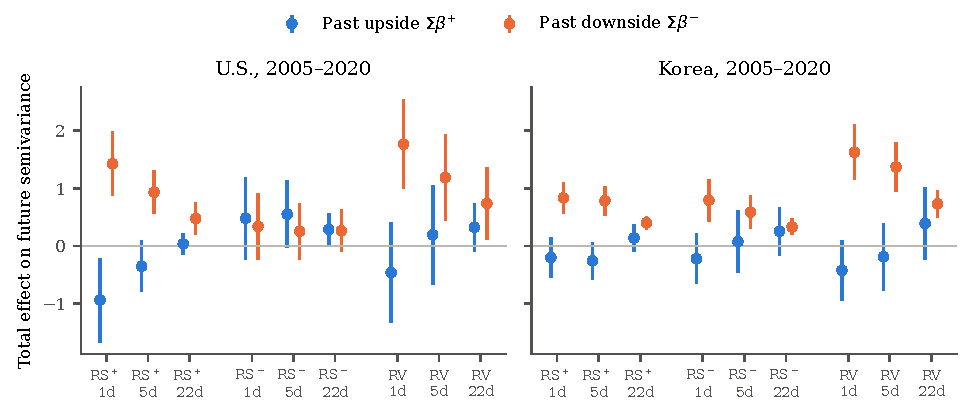
\includegraphics[width=\textwidth]{figures/fig_semivar.pdf}
\caption{Total effects of past upside and downside semivariance on future semivariance, development sample. Points are $\Sigma\beta^{+}$ and $\Sigma\beta^{-}$; bars are 95\% Newey--West confidence intervals.}\label{fig:semivar}
\end{figure}

\begin{table}[!htbp]
\centering
\begin{threeparttable}
\caption{Total effects of past upside and downside semivariance}\label{tab:semivar}
\scriptsize
\begin{tabular}{lcccccc}
\toprule
 & \multicolumn{3}{c}{U.S.} & \multicolumn{3}{c}{Korea} \\
\cmidrule(lr){2-4}\cmidrule(lr){5-7}
Target, horizon & $\Sigma\beta^{+}$ & $\Sigma\beta^{-}$ & $\Sigma\beta^{-}-\Sigma\beta^{+}$ & $\Sigma\beta^{+}$ & $\Sigma\beta^{-}$ & $\Sigma\beta^{-}-\Sigma\beta^{+}$ \\
\midrule
\inputtable{tables/t_semivar.tex}
\bottomrule
\end{tabular}
\begin{tablenotes}\footnotesize
\item Estimates with Newey--West $t$-statistics in parentheses. $^{\dagger}$: Holm-adjusted $p<0.05$ within the family of 27 tests for the given market and sample. Holm-significant tests per family (U.S.\ dev, Korea dev, U.S.\ test, Korea test): 7/27, 13/27, 11/27, 0/27.
\end{tablenotes}
\end{threeparttable}
\end{table}

\subsection{Does the leverage effect strengthen in turbulent regimes?}

We classify each day as calm or turbulent with an online statistical jump model fitted to volatility features \citep{nystrup2020}, following the regime-switching application of \citet{shu2024}, re-estimated monthly on past data only. The turbulent regime covers 25.5\% of days in the U.S.\ and 12.2\% in Korea, with annualized volatility of 33.5\% and 39.5\%, respectively; online and full-sample classifications agree on 96.7\% and 94.3\% of days (Appendix Table~\ref{tab:regime}). The Korean indicator captures only large crises: it classified none of the 2015--16 China shock or the fourth quarter of 2018 as turbulent. Adding the regime dummy and its interactions to LHAR (RLHAR; Table~\ref{tab:coef}), the coefficient on $L_t\times D_t$ is $-0.216$ ($t=-4.62$) in the U.S.\ and $-0.045$ ($t=-1.47$) in Korea. The effect of a one-point decline on log variance thus falls from 0.245 in calm periods to about 0.03 in turbulent periods in the U.S.: when volatility is already elevated, a further decline adds little. Regime information improves forecasts modestly (QLIKE 1.4\% and 1.1\% below LHAR, DM $t\approx2.0$), through the level and persistence terms rather than through the decline term, and the improvement is not significant after Holm adjustment ($p=0.13$).\footnote{A preliminary estimate in our own analysis had the opposite sign. It regressed the level of $RV_{t+1}$ on log regressors, a specification that differs from the log model used for forecasting. The out-of-sample comparisons were unaffected.}

\begin{table}[!htbp]
\centering
\begin{threeparttable}
\caption{LHAR and regime-LHAR coefficients, development sample}\label{tab:coef}
\scriptsize
\begin{tabular}{lcccc}
\toprule
 & \multicolumn{2}{c}{U.S.} & \multicolumn{2}{c}{Korea} \\
\cmidrule(lr){2-3}\cmidrule(lr){4-5}
 & LHAR & RLHAR & LHAR & RLHAR \\
\midrule
\inputtable{tables/t_coef.tex}
\bottomrule
\end{tabular}
\begin{tablenotes}\footnotesize
\item Dependent variable $\log RV_{t+1}$. Newey--West $t$-statistics (22 lags) in parentheses. $^{*}$, $^{**}$, $^{***}$: $p<0.05$, $0.01$, $0.001$ (unadjusted). $D_t$ is the online turbulent-regime indicator.
\end{tablenotes}
\end{threeparttable}
\end{table}

% ===========================================================================
\section{Daily directional asymmetry measures and short-term reversal}\label{sec:skew}
% ===========================================================================

\subsection{Monthly relative signed jump variation}

For each stock and month we compute RSJ $=(RS^{+}-RS^{-})/RV$ and realized skewness from daily returns, together with maximum daily return (MAX), idiosyncratic volatility (IVOL), and the monthly return (REV). Table~\ref{tab:rsj} shows that RSJ has a rank correlation of 0.85 (U.S.) and 0.87 (Korea) with the same-month return. In the U.S., RSJ alone has a significant Fama--MacBeth coefficient ($t=-2.08$) that turns positive and insignificant once REV is added, and a double sort on RSJ within REV quintiles yields no spread. None of the five candidate signals met our pre-specified selection criteria (neutralized IC $|t|\ge2$, same sign in both halves, monotone quintiles, positive long leg) in either market, and none of the 30 tests in this family is significant even before adjustment. Signal effects do not differ significantly between calm and turbulent months or between the two countries after adjustment (Table~\ref{tab:mt}); the only robust regime effect is that the cross-sectional dispersion of returns rises in turbulent months in the U.S.\ (Holm $p=0.005$).

\begin{table}[!htbp]
\centering
\begin{threeparttable}
\caption{Monthly RSJ and short-term reversal, 2010--2020}\label{tab:rsj}
\small
\begin{tabular}{lcc}
\toprule
 & U.S. & Korea \\
\midrule
\inputtable{tables/t_rsj.tex}
\bottomrule
\end{tabular}
\begin{tablenotes}\footnotesize
\item Monthly rank ICs and Fama--MacBeth coefficients with Newey--West $t$-statistics (3 lags) in parentheses. Neutralized IC removes REV, MAX, IVOL, RSkew, size, illiquidity, and momentum. U.S.\ results refer to surviving large-capitalization stocks.
\end{tablenotes}
\end{threeparttable}
\end{table}

\subsection{Weekly realized skewness}

Following the design of \citet{amaya2015} as closely as our data allow, we compute each stock's realized skewness from the week's daily returns, sort stocks into deciles at the end of each week, and hold the lowest-minus-highest decile portfolio for the next week. The design was frozen before any result was computed.

Table~\ref{tab:skew} and Figure~\ref{fig:deciles} report the results. In the development sample the spread has the sign documented by \citet{amaya2015}: 14.0 bps per week in the U.S.\ ($t=1.90$) and 21.0 bps (equal-weighted) and 46.8 bps (value-weighted, $t=4.19$) in Korea. But skewness from five daily returns is essentially a re-measurement of the week's return: its average weekly rank correlation with the same-week return is 0.760 (U.S.) and 0.816 (Korea), compared with about 0.3 for skewness computed over the past 22 trading days. With the 22-day measure, which is less entangled with the week's return, the gross long--short spread is insignificant in every sample (Appendix Table~\ref{tab:skew22}). In Fama--MacBeth regressions, the skewness coefficient ($-6.35$ and $-10.96$ bps per standard deviation) falls to $-0.25$ ($p=0.88$) and $-2.84$ ($p=0.33$) once the week's return, volatility, and size are controlled for, while the reversal coefficient is significant. After Holm adjustment only the Korean value-weighted spread and the Korean skewness-only coefficient remain significant in the development sample; nothing is significant in the test sample, with or without the months of the Korean short-sale ban (Appendix Table~\ref{tab:banrobust}).

The strategy turns over about 360\% of its (two-leg) value each week, so costs erase the development-sample spread in the U.S.\ and turn it into a loss of 47 bps per week in Korea, where the transaction tax is levied on every sale. A long-only version that buys the lowest-skewness decile underperforms the equal-weighted universe in both markets.

We emphasize the scope of this result. \citet{amaya2015} compute skewness from about 390 five-minute returns per week for the full CRSP universe, and \citet{sim2016} likewise uses intraday data for Korea. Our 60-minute version for 50 large stocks over three years shows no effect either (U.S.\ $-4.5$ bps, $p=0.86$; Korea $-7.0$ bps, $p=0.81$), but it has little power. Our evidence shows that the \emph{daily approximation} of realized skewness cannot be distinguished from short-term reversal; it neither confirms nor refutes the high-frequency result.

\begin{table}[!htbp]
\centering
\begin{threeparttable}
\caption{Weekly realized skewness from daily returns}\label{tab:skew}
\scriptsize
\begin{tabular}{lcccc}
\toprule
 & \multicolumn{2}{c}{U.S.} & \multicolumn{2}{c}{Korea} \\
\cmidrule(lr){2-3}\cmidrule(lr){4-5}
 & 2010--2020 & 2021--2026 & 2010--2020 & 2021--2026 \\
\midrule
\inputtable{tables/t_skew.tex}
\bottomrule
\end{tabular}
\begin{tablenotes}\footnotesize
\item Long--short is decile 1 (lowest skewness) minus decile 10. Net returns deduct one-way costs and the Korean sell-side tax; short-borrowing costs are not deducted. Newey--West $t$-statistics (4 lags) in parentheses. $^{\dagger}$: Holm-adjusted $p<0.05$ within the family of 24 tests for the sample (gross long--short, long-only, and Fama--MacBeth skewness coefficients for both markets and both skewness windows). The universe row and net long--short rows are not part of the family.
\end{tablenotes}
\end{threeparttable}
\end{table}

\begin{figure}[!htbp]
\centering
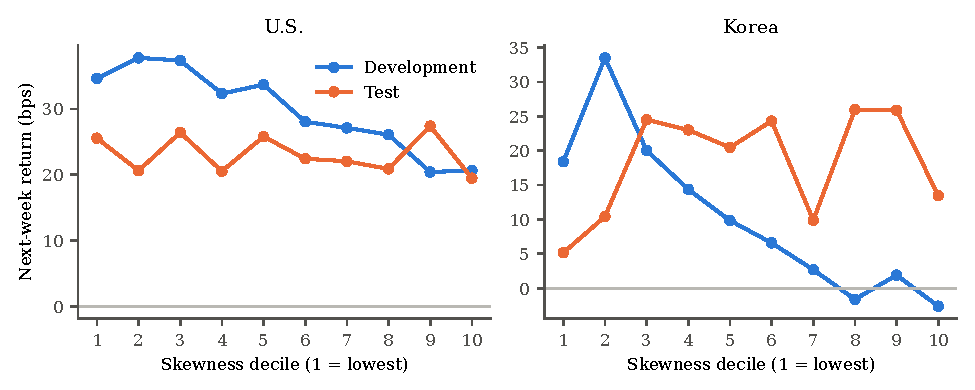
\includegraphics[width=\textwidth]{figures/fig_skew_deciles.pdf}
\caption{Next-week equal-weighted returns of weekly skewness deciles (bps).}\label{fig:deciles}
\end{figure}

% ===========================================================================
\section{Magnitude is predictable, direction is not}\label{sec:direction}
% ===========================================================================

\subsection{The dominant direction of index variation}

Let $s_t=RS^{+}_t/(RS^{+}_t+RS^{-}_t)$ be the upside share of variation over a window of $k$ days, measured from daily or intraday (60-, 10-, 5-minute) returns. We regress the future share over $h$ days on the past share and compare the hit rate of a ``reversal'' rule (predict the opposite of the past dominant direction) with a baseline that always predicts the sample majority.

Across 84 specifications, 10 coefficients are significant before adjustment and all 10 have the reversal sign, but only one survives Holm adjustment: the U.S.\ daily index in the development sample ($\beta=\dirBeta$). Even there the reversal rule hits \dirHit\% of days against \dirBase\% for the baseline, and the coefficient vanishes in the test sample ($\beta=\dirBetaTest$, $p=\dirPTest$). The reversal rule never beats the baseline significantly and is significantly worse in 24 cases. Apparent regime dependence and post-crash rebounds do not survive adjustment either (Table~\ref{tab:direction}).

\begin{table}[!htbp]
\centering
\begin{threeparttable}
\caption{Forecasting the dominant direction of variation: summary of tests}\label{tab:direction}
\small
\begin{tabular}{lccccc}
\toprule
Family & Tests & $p<0.05$ & Holm & BH & $|t|>3$ \\
\midrule
\inputtable{tables/t_direction.tex}
\bottomrule
\end{tabular}
\begin{tablenotes}\footnotesize
\item Each family pools daily and intraday data, both markets, and (for daily data) both samples. Significant hit-rate tests are all cases in which the reversal rule is \emph{worse} than the baseline.
\end{tablenotes}
\end{threeparttable}
\end{table}

\subsection{Stock-level upside and downside forecasts}

We forecast each stock's next-month upside and downside semivariance with a pooled regression on its own daily, weekly, and monthly semivariances, re-estimated monthly on realized data only. Table~\ref{tab:s4} (Panel A) shows that both forecasts are informative about magnitude (average cross-sectional rank correlation 0.43--0.57 with realized values) but that they rank stocks almost identically (0.98--0.997). The predicted upside share has a rank correlation of only 0.03 with the realized share in the U.S.\ and is negative in Korea. The reason is that realized semivariance factors into a persistent magnitude and a transient share: the magnitude carries over to the next month, the share does not.

A frozen strategy (S4) that buys stocks with high predicted upside semivariance and sells them when the predicted upside-to-downside ratio deteriorates does not significantly outperform the equal-weighted universe or the index ETF in either sample (Panel B). In Korea, stocks with a high predicted upside share subsequently \emph{underperformed} (test-sample IC $-0.077$, $t=-4.09$). This pattern was found after the fact and we do not treat it as evidence.

\begin{table}[!htbp]
\centering
\begin{threeparttable}
\caption{Stock-level semivariance forecasts and the S4 strategy}\label{tab:s4}
\scriptsize
\begin{tabular}{lcccc}
\toprule
\multicolumn{5}{l}{\textit{Panel A: Average monthly cross-sectional rank correlation}}\\
 & \multicolumn{2}{c}{U.S.} & \multicolumn{2}{c}{Korea} \\
\cmidrule(lr){2-3}\cmidrule(lr){4-5}
 & Dev. & Test & Dev. & Test \\
\midrule
\inputtable{tables/t_s4_forecast.tex}
\midrule
\multicolumn{5}{l}{\textit{Panel B: Frozen S4 minus benchmark, annualized \% (Newey--West $t$) and Holm $p$}}\\
 & \multicolumn{2}{c}{Development} & \multicolumn{2}{c}{Test} \\
\cmidrule(lr){2-3}\cmidrule(lr){4-5}
 & Diff. & Holm $p$ & Diff. & Holm $p$ \\
\midrule
\inputtable{tables/t_s4_excess.tex}
\bottomrule
\end{tabular}
\begin{tablenotes}\footnotesize
\item Korean stock returns exclude dividends whereas the ETF includes them, which biases the Korea S4 $-$ ETF comparison against S4 by roughly the dividend yield. U.S.\ results refer to surviving large-capitalization stocks; missing forward returns are set to zero.
\end{tablenotes}
\end{threeparttable}
\end{table}

% ===========================================================================
\section{The 2023--2025 Korean short-sale ban}\label{sec:ban}
% ===========================================================================

Korea banned all short selling from November 2023 to March 2025. If short-sale constraints slow the incorporation of negative information, the cross-sectional pricing of asymmetry and lottery-type measures could change during the ban. For each signal $S\in\{\text{RSJ},\text{RSkew},\text{IVOL},\text{MAX}\}$ we estimate monthly Fama--MacBeth slopes $b^{KR}_t$ and $b^{US}_t$ controlling for REV and size, and regress their difference on ban and post-ban indicators and the two countries' regime indicators,
\begin{equation}
b^{KR}_t-b^{US}_t=\theta_0+\theta_3\,\text{Ban}_t+\theta_4\,\text{Post}_t+\delta_1 D^{KR}_t+\delta_2 D^{US}_t+u_t .
\end{equation}
Differencing removes global shocks common to both markets in the same month.

Table~\ref{tab:ban} shows no significant ban effect for any signal ($|t|\le1.35$). We compare $\theta_3$ with a placebo distribution obtained by moving a 17-month fake ban through the 2010--2020 sample. Because that sample contains two actual Korean bans (August--November 2011 and March 2020 to April 2021),\footnote{Short selling resumed in May 2021 only for constituents of the KOSPI 200 and KOSDAQ 150; other stocks remained under the ban until it was extended to all stocks in November 2023. Our Korean universe, the 200 largest KOSPI common stocks by market capitalization, approximates the KOSPI 200, so we treat April 2021 as the end of that ban; a few stocks near the size cutoff may have remained unshortable. \citet{kimkim2024} exploit exactly this index-membership rule to study the 2021 partial reopening. Financial stocks were also under a ban from October 2008 to November 2013, which overlaps the first placebo years for that sector only.} we drop those months and all placebo windows that span them, which reduces the number of placebo windows from \nPlaceboOld{} to \nPlaceboNew{}; excluding the same months from the main regression leaves the estimates unchanged. Placebo $p$-values range from 0.15 to 0.70 (Figure~\ref{fig:placebo}). Excluding February 2024 (the announcement of the ``Value-up'' program) and December 2024 (martial-law turmoil) also changes nothing.

Three caveats limit the interpretation. First, the pre-ban slopes of these signals were close to zero (Section~\ref{sec:skew}), so there was little to change and the test has low power. Second, a within-Korea design comparing stocks with high and low pre-ban short interest would be more direct, but stock-level short-interest data were not available to us through the KRX Open API, so we do not pursue it. Third, the U.S.\ is an imperfect control for Korea-specific shocks.

\begin{table}[!htbp]
\centering
\begin{threeparttable}
\caption{Cross-country difference-in-differences: the Korean short-sale ban}\label{tab:ban}
\scriptsize
\begin{tabular}{lcccccc}
\toprule
 & \multicolumn{3}{c}{Full sample} & \multicolumn{2}{c}{Excluding prior bans} & Excl.\ events \\
\cmidrule(lr){2-4}\cmidrule(lr){5-6}\cmidrule(lr){7-7}
Signal & $\theta_3$ ($t$) & Placebo $p$ (orig.) & Placebo $p$ (purged) & $\theta_3$ ($t$) & Placebo $p$ & $\theta_3$ ($t$) \\
\midrule
\inputtable{tables/t_ban.tex}
\bottomrule
\end{tabular}
\begin{tablenotes}\footnotesize
\item $\theta_3$ is the ban coefficient with Newey--West $t$-statistics (3 lags). ``Orig.'' uses all \nPlaceboOld{} placebo windows in 2010--2020; ``purged'' drops months of the 2011 and 2020--2021 Korean bans and windows spanning them (\nPlaceboNew{} windows). ``Excluding prior bans'' also drops those months from the main regression. ``Excl.\ events'' drops February and December 2024.
\end{tablenotes}
\end{threeparttable}
\end{table}

\begin{figure}[!htbp]
\centering
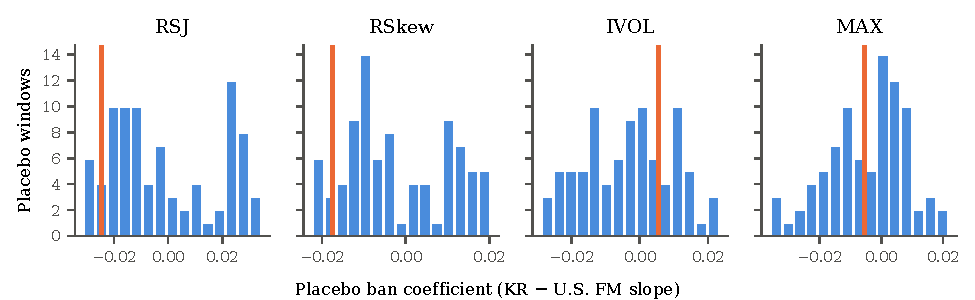
\includegraphics[width=\textwidth]{figures/fig_placebo.pdf}
\caption{Purged placebo distributions of the ban coefficient (bars) and the actual estimate excluding prior bans (vertical line).}\label{fig:placebo}
\end{figure}

% ===========================================================================
\section{Implications for practice}\label{sec:practice}
% ===========================================================================

If volatility is predictable but returns are not, volatility forecasts are best used to size positions. Table~\ref{tab:timing} compares two frozen allocation rules on the index ETFs: a regime switch that holds the ETF in calm regimes and cash in turbulent ones (S1\_A), and volatility targeting that scales exposure by the ratio of a target to forecast volatility (S1v2).

The regime switch had the highest development-sample Sharpe ratio in the U.S.\ (0.71, maximum drawdown $-15\%$ against $-55\%$ for buy-and-hold) but the lowest test-sample Sharpe ratio in both markets, below a 200-day moving-average rule. Table~\ref{tab:turbulent} explains why. In 2005--2020, turbulent days in the U.S.\ earned roughly the same average return as calm days with much higher risk, so avoiding them cut risk at little cost; in Korea they were rare (8\% of days). In 2021--2026, turbulent days earned the \emph{highest} returns---21.6\% annualized in the U.S.\ and 69.0\% in Korea---because sharp rebounds after the 2022 drawdown, August 2024, and April 2025, as well as much of the 2025--2026 Korean rally, coincided with high-volatility periods. Exiting the market forfeited them. Selection among several candidate rules on the development sample adds a winner's-curse component.

Volatility targeting, which reduces but never eliminates exposure, delivered Sharpe ratios close to or above buy-and-hold in both periods with lower volatility and drawdowns. None of its test-period differences from buy-and-hold, the moving-average rule, naive volatility targeting, or the regime switch is significant after adjustment (all Holm $p\ge0.63$). Excluding the months of the Korean short-sale ban raises every Korean Sharpe ratio and lowers every U.S.\ one, since those months were weak for Korea and strong for the U.S., but volatility targeting still has the highest and the regime switch the lowest Sharpe ratio in Korea, and the difference between volatility targeting and buy-and-hold remains insignificant in both markets (Appendix Table~\ref{tab:banrobust}). A more elaborate forecast (adding upside semivariance or a 22-day horizon) did not improve meaningfully on naive 22-day realized volatility even in the development sample: the four candidate forecasts and the naive rule differ by at most 0.06 in Sharpe ratio, against standard errors of about 0.3. The test-period results for S1v2 are contaminated because a closely related rule had been evaluated on the same period before S1v2 was designed; its validation relies on paper trading that started in September 2026.

\begin{table}[!htbp]
\centering
\begin{threeparttable}
\caption{Allocation rules on index ETFs}\label{tab:timing}
\scriptsize
\begin{tabular}{lcccccc}
\toprule
 & \multicolumn{2}{c}{Development} & \multicolumn{4}{c}{Test (2021--2026)} \\
\cmidrule(lr){2-3}\cmidrule(lr){4-7}
 & Sharpe & MDD (\%) & Return (\%) & Sharpe & s.e. & MDD (\%) \\
\midrule
\inputtable{tables/t_timing.tex}
\bottomrule
\end{tabular}
\begin{tablenotes}\footnotesize
\item Daily rebalancing with a one-day execution lag, a 10-point no-trade band for volatility-targeting rules, and one-way ETF costs. U.S.\ cash earns the 3-month T-bill rate; Korean cash earns zero. The development sample is 2005--2020 for the U.S.\ and about 11.5 years for Korea (the ETF starts in 2007). All strategies are evaluated on common dates.
\end{tablenotes}
\end{threeparttable}
\end{table}

\begin{table}[!htbp]
\centering
\begin{threeparttable}
\caption{ETF returns on turbulent and calm days}\label{tab:turbulent}
\small
\begin{tabular}{llcccc}
\toprule
Market & Period & Turbulent days (\%) & Turbulent (ann.\ \%) & Calm (ann.\ \%) & Cumulative on turbulent days (\%) \\
\midrule
\inputtable{tables/t_turbulent.tex}
\bottomrule
\end{tabular}
\begin{tablenotes}\footnotesize
\item Days are classified by the previous day's online regime. Annualized arithmetic mean returns.
\end{tablenotes}
\end{threeparttable}
\end{table}

% ===========================================================================
\section{Conclusion}\label{sec:conclusion}
% ===========================================================================

Asymmetric volatility is real and useful: downside semivariance forecasts future volatility in both Korea and the U.S., the result survives multiple-testing adjustment, and it replicates out of sample in the U.S. It is not, however, a source of return predictability in our data. Daily-frequency directional asymmetry measures are statistically indistinguishable from short-term reversal, the direction of future variation cannot be forecast, stock-level upside and downside forecasts collapse into a single magnitude forecast, and the 2023--2025 Korean short-sale ban left the cross-sectional pricing of these measures unchanged. In practice, the information is better used to scale risk than to pick stocks or time the market.

Our study has clear limitations: the U.S.\ cross-section is a survivor sample; Korean stock returns exclude dividends and the tax schedule is simplified; intraday samples are short; the short-sale analysis lacks a within-Korea design; and our freezing protocol is internal. Future work should test the overnight--intraday decomposition in Appendix~\ref{app:overnight} on a longer intraday sample, examine whether the saturation of the leverage effect holds in other markets, and evaluate high-frequency realized skewness on the full Korean cross-section.

\section*{Data and code availability}

The code that downloads the data, constructs all variables, runs every analysis, freezes rule sets, and generates the tables and figures of this paper is available at \url{https://github.com/caxios/downside-volatility-korea-us}. The repository also contains the five frozen rule files with their SHA-256 hashes, the complete log of test-period data access, the paper-trading records, and every result table from which the tables and figures of this paper are built; a script recomputes the hashes and lists the logged accesses. These files were kept locally until the repository was made public, so the repository provides the first external record of them. Raw data are not redistributed: index, ETF, U.S.\ stock, and intraday prices were obtained from Yahoo Finance, Korean stock data from the Korea Exchange Open API (\url{https://openapi.krx.co.kr}; non-commercial use, redistribution not permitted), Fama--French factors from Kenneth French's data library, and the U.S.\ Treasury bill rate from FRED. The download scripts reproduce the data set subject to the providers' terms and to revisions of the source data.

\section*{Declaration of generative AI use}

This paper was prepared with extensive use of Claude Code (Anthropic), an AI coding assistant based on Claude large language models, between September 15 and September 30, 2026. The assistant wrote all of the code in the replication package, ran every analysis, contributed to aspects of the empirical design and the robustness checks, drafted the working reports and this manuscript. The author set the research agenda, suggested bibliographic references, directed the empirical design and robustness checks, supported by Claude, made the decisions on scope, data sources, and code release, and performed the corrections and checks reported in the paper. Several errors in the assistant's earlier output were found and corrected during the project; those that affected reported results are noted in the paper. The author verified every reference against the original source, read the full manuscript, checked the compiled output, and takes full responsibility for the content. The AI tool is not an author of this paper.

\bibliographystyle{plainnat}
\bibliography{references}

\clearpage
\appendix

% ===========================================================================
\section{Audit trail}\label{app:audit}
% ===========================================================================

\begin{table}[!htbp]
\centering
\caption{Frozen rule sets}\label{tab:frozen}
\small
\begin{tabular}{llll}
\toprule
Rule set & Frozen at & SHA-256 (first 12) & Content \\
\midrule
S1 & 2026-09-27 09:32:48 & \texttt{c6bf0fe3c487} & Regime switch, JM $\lambda=5$ \\
S2S3 & 2026-09-28 15:18:51 & \texttt{44136fa355b3} & Empty (no signal selected) \\
S4 & 2026-09-28 21:44:08 & \texttt{84a1faf3991e} & Semivariance stock selection \\
S5 & 2026-09-29 13:42:08 & \texttt{292324739ed3} & Weekly skewness design \\
S1v2 & 2026-09-29 21:06:20 & \texttt{a4a0323a5979} & Volatility targeting variant \\
\bottomrule
\end{tabular}
\end{table}

\noindent Test-period access (from the project log): S1 final test 4 minutes after freezing; cross-country ban analysis and intraday validation 15 seconds and 1 minute after freezing S2S3; daily semivariance replication (three runs) and intraday semivariance (three runs) on 2026-09-28 without a frozen specification; S4 test 12 seconds after freezing (run twice to store monthly returns, identical results); an ad hoc check of the direction analysis two minutes before its formal run on 2026-09-29; S5 tests 10--35 minutes after freezing; S1v2 test about 30 seconds after freezing; the purged-placebo re-estimation of the ban analysis on 2026-09-29; and the short-sale-ban robustness check (Table~\ref{tab:banrobust}) on 2026-09-30, run three times while its code was debugged, which re-uses the S1v2 test code and therefore also appears in the log under the S1v2 label. No frozen rule was changed by these checks. The full log and hash files are part of the replication package.

% ===========================================================================
\section{Multiple-testing summary}\label{app:mt}
% ===========================================================================

\begin{table}[!htbp]
\centering
\begin{threeparttable}
\caption{Multiple-testing adjustments by set of results}\label{tab:mt}
\small
\begin{tabular}{lcccccc}
\toprule
Set of results & Families & Tests & $p<0.05$ & Holm & BH & $|t|>3$ \\
\midrule
\inputtable{tables/t_mt.tex}
\bottomrule
\end{tabular}
\begin{tablenotes}\footnotesize
\item Counts of tests significant at 5\% before adjustment, after Holm (FWER) and Benjamini--Hochberg (FDR) adjustment within families, and with $|t|>3$. Families are defined by hypothesis (main results), by market and sample (daily semivariance, S4, S5), by data set (intraday), and by type of test (direction).
\end{tablenotes}
\end{threeparttable}
\end{table}

% ===========================================================================
\section{Exploratory evidence: intraday versus overnight}\label{app:overnight}
% ===========================================================================

In 60-minute data, the difference $\Sigma\beta^{-}-\Sigma\beta^{+}$ between the total effects of intraday downside and upside semivariance is insignificant for the U.S.\ index and for both 50-stock panels; in the Korean panel both total effects are significant and of similar size. When intraday and overnight (close-to-open) semivariances enter the same regression for the U.S.\ index, the downside--upside difference is positive for overnight moves at all horizons with unadjusted $p$-values of 0.02--0.03 (Table~\ref{tab:overnight}). This pattern suggests that the daily asymmetry may originate in overnight gaps, but it does not survive adjustment within the 54 tests of the decomposition (Holm $p=1.0$, BH $p=0.135$), the sample covers only about three years, and the Korean index shows the opposite pattern in an extreme market. We therefore report it only as a hypothesis for future work.

\begin{table}[!htbp]
\centering
\begin{threeparttable}
\caption{Intraday--overnight decomposition, U.S.\ index, 60-minute bars (2023--2026)}\label{tab:overnight}
\small
\begin{tabular}{lcccccc}
\toprule
Block & $h$ & $\Sigma\beta^{-}-\Sigma\beta^{+}$ & $t$ & $p$ & Holm $p$ & BH $p$ \\
\midrule
\inputtable{tables/t_overnight.tex}
\bottomrule
\end{tabular}
\begin{tablenotes}\footnotesize
\item Target is future total intraday variance. Newey--West standard errors.
\end{tablenotes}
\end{threeparttable}
\end{table}

% ===========================================================================
\section{Robustness}\label{app:robust}
% ===========================================================================

\begin{table}[!htbp]
\centering
\begin{threeparttable}
\caption{Regime model diagnostics, development sample}\label{tab:regime}
\small
\begin{tabular}{lcc}
\toprule
 & U.S. & Korea \\
\midrule
\inputtable{tables/t_regime.tex}
\bottomrule
\end{tabular}
\begin{tablenotes}\footnotesize
\item Two-state statistical jump model on volatility features (half-lives 5, 10, 21 days), re-estimated monthly on past data and filtered online. $\lambda$ was chosen from five candidates by the development-sample Sharpe ratio of the regime-switch rule. Agreement with a two-state Gaussian HMM (filtered probability $>0.5$) is a robustness check. Event windows follow the definitions in the replication code.
\end{tablenotes}
\end{threeparttable}
\end{table}

\begin{table}[!htbp]
\centering
\begin{threeparttable}
\caption{Semivariance total effects after winsorizing, development sample}\label{tab:winsor}
\scriptsize
\begin{tabular}{lcccccc}
\toprule
 & \multicolumn{3}{c}{U.S.} & \multicolumn{3}{c}{Korea} \\
\cmidrule(lr){2-4}\cmidrule(lr){5-7}
Target, horizon & $\Sigma\beta^{+}$ & $\Sigma\beta^{-}$ & $\Sigma\beta^{-}-\Sigma\beta^{+}$ & $\Sigma\beta^{+}$ & $\Sigma\beta^{-}$ & $\Sigma\beta^{-}-\Sigma\beta^{+}$ \\
\midrule
\inputtable{tables/t_winsor.tex}
\bottomrule
\end{tabular}
\begin{tablenotes}\footnotesize
\item As Table~\ref{tab:semivar}, Panel A, with regressors and targets winsorized at the 99.5th percentile. $^{*}$, $^{**}$, $^{***}$: unadjusted $p<0.05$, $0.01$, $0.001$ (Newey--West).
\end{tablenotes}
\end{threeparttable}
\end{table}

\begin{table}[!htbp]
\centering
\begin{threeparttable}
\caption{Realized skewness over the past 22 trading days}\label{tab:skew22}
\scriptsize
\begin{tabular}{lcccc}
\toprule
 & \multicolumn{2}{c}{U.S.} & \multicolumn{2}{c}{Korea} \\
\cmidrule(lr){2-3}\cmidrule(lr){4-5}
 & 2010--2020 & 2021--2026 & 2010--2020 & 2021--2026 \\
\midrule
\inputtable{tables/t_skew22.tex}
\bottomrule
\end{tabular}
\begin{tablenotes}\footnotesize
\item As Table~\ref{tab:skew}, with skewness computed from the 22 daily returns ending on the portfolio formation day. Returns in bps per week; Fama--MacBeth coefficients in bps per standard deviation. Newey--West $t$-statistics in parentheses. Controls: REV, RVOL, SIZE.
\end{tablenotes}
\end{threeparttable}
\end{table}

\begin{table}[!htbp]
\centering
\begin{threeparttable}
\caption{Test sample excluding the 2023--2025 Korean short-sale ban}\label{tab:banrobust}
\scriptsize
\begin{tabular}{lcccc}
\toprule
 & \multicolumn{2}{c}{U.S.\ (calendar control)} & \multicolumn{2}{c}{Korea} \\
\cmidrule(lr){2-3}\cmidrule(lr){4-5}
 & Full & Excl.\ ban & Full & Excl.\ ban \\
\midrule
\inputtable{tables/t_ban_robust.tex}
\bottomrule
\end{tabular}
\begin{tablenotes}\footnotesize
\item Test sample, January 2021 to September 2026. ``Excl.\ ban'' drops November 2023 to March 2025 in both markets; frozen rules and parameters are unchanged. Panel A drops every day whose regressor window (past 22 days) or target window overlaps the ban; Holm adjustment within the 27 tests of each market and sample, as in Table~\ref{tab:semivar}. Panel B drops weeks whose holding week overlaps the ban; Panel C drops ban months. Panel D: net daily returns on the dates common to all strategies; the S1v2 difference from buy-and-hold and the QLIKE comparison (Diebold--Mariano $t$) use Newey--West $t$-statistics. Full-sample Korean Sharpe ratios can differ from Table~\ref{tab:timing} in the third decimal because of a later data refresh. $t$-statistics in parentheses are not adjusted for multiple testing; the U.S.\ columns serve only to separate the effect of the ban from that of the calendar period.
\end{tablenotes}
\end{threeparttable}
\end{table}

\end{document}
